\chapter{Event simulation and reconstruction} \label{chp:labelTitle}

An accurate understanding of simulated events and their reconstruction is crucial for a thorough understanding of the collected data. Hence event generators such as $\Madgraph$, $\Pythia$ and $\Herwig$ play the role of hadron colliders and allow some improvement of analyzing power by using an efficient background and signal discriminator.

\section{QCD for hadron colliders} \label{sec::QCDHadron}

The composite nature of protons together with the high-momentum transfers reachable \textit{(conceivable)} at the LHC significantly complicates the event structure. 
Hence for a thorough understanding of the different processes taking place during the generation of a single proton-proton collision it is factorized into separate steps.
An overview of this factorization is shown in Figure~\ref{fig::EvtShower} with the different stages briefly discussed below.

\begin{figure}[htb]
 \centering
 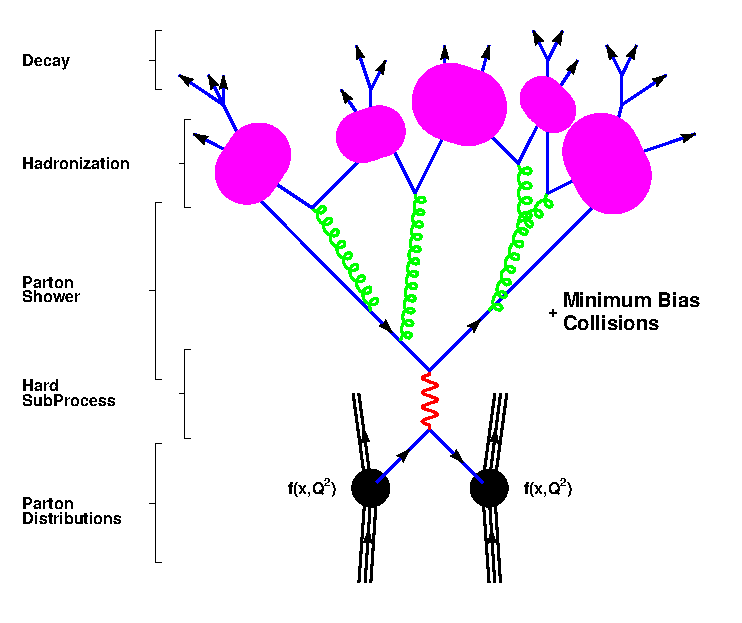
\includegraphics[width = 0.8 \textwidth]{Chapters/Chapter3/Figures/f_shg_event.eps}
 \caption{Schematical overview of the consecutive steps of the event generation process.}  \label{fig::EvtShower}
\end{figure}

\begin{myindentpar}
  \begin{description}
    \item[Parton Distribution Functions] \hfill \\
      In proton-proton collisions both incoming protons can be viewed as a collection of partons whose momentum fraction $x$ within the hadron is parametrized by the so-called parton distribution functions.
    \item[Hard scattering] \hfill \\
      Hard scattering is the perturbative process of two colliding partons, one originating from each proton, that creates high-energetic particles. It can be represented by a factorized product of short-and long-distance contributions as discussed in Section~\ref{sec::HardScattering}.
    \item[Parton shower] \hfill \\
      This phase of the event generation process describes the approximate higher-order corrections induced by emission of additional gluon and/or quarks, as will be explained in Section~\ref{sec::PS}. Depending whether this radiation originates from the incoming or outgoing partons it is denominated, respectively, Initial State Radiation (ISR) or Final State Radiation (FSR).
    \item[Hadronisation] \hfill \\
      The collection of \textit{(receding)} post-shower partons is combined into experimentally observable colour-neutral hadrons as required by colour confinement. This hadronisation process is described by QCD-inspired phenomenological models as discussed in Section~\ref{sec::Hadronisation}.
    %\item[Underlying event (why is this a separate item? Doesn't show up in the schematical overview ...)] \hfill \\
  \end{description}
\end{myindentpar}

The main challenge at hadron colliders \textit{(compared to lepton colliders)} is the missing information about the partons responsible for the hard interaction. 
The event generation process at the LHC is even more arduous due to the QCD activity in a widespread range of involved momentum transfer. %, according to the scale of momentum transfer involved. 
The interaction starts at a scale of barely $1$ $\GeV$ with partons confined in a proton beam, then produces during the hard interaction a few high-energetic outgoing leptons, gauge bosons or partons of which the latter afterwards transform non-perturbatively into final-state hadrons. This large variation in energy range, and corresponding QCD coupling strength, implies that only the high-momentum transfer part of the event generation can be derived exactly from the QCD Lagrangian while the other aspects have to be expressed using phenomenological non-perturbative models.

\subsection{Hard Scattering (=? Jet Fragmentation)} \label{sec::HardScattering}
Most events studied at the LHC involve high-momentum transfers in order to create massive particles or high-energetic jets. The inclusive production cross section of an observable $X$ from hadrons $h_1$ and $h_2$ for these type of interactions can be factorized into:

%Due to the internal structure of the protons, the inclusive cross section $\sigma_{h_{1}h_{2} \rightarrow X}$ cannot be calculated exactly from first principles but has to be factorized in terms of the partonic scattering cross section $\hat{\sigma}_{ab \rightarrow X}$ and the parton distribution functions $f_{a}^{h}$. Therefore, within the collinear limit~\cite{ColLimit}, the inclusive cross section for $X$-production can be written as:
%\\ \textit{Should check whether there is a difference between $\hat{\sigma}_{ab \rightarrow X}$ and $\hat{\sigma}(\Phi_{ab \rightarrow X},\mu^{2}_{F})$??}
\begin{equation} \label{eq::HSXS}
 \sigma_{h_{1}h_{2} \rightarrow X} =\sum_{a,b \in \{q,g\} } \int dx_{a} \int dx_{b} f_{a}^{h_{1}}(x_{a},\mu^{2}_{F}) f_{b}^{h_{2}}(x_{b},\mu^{2}_{F}) \int d\Phi_{ab \rightarrow X} \dfrac{d\hat{\sigma}(\Phi_{ab \rightarrow X},\mu^{2}_{F})}{d\Phi_{ab \rightarrow X}}
\end{equation}
From Equation~(\ref{eq::HSXS}) can be concluded that the hadronic cross section, valid for all orders in perturbation theory, is actually a convolution of a perturbatively short-distance component $\hat{\sigma}_{ab \rightarrow X}$, calculable from Matrix Elements, and an approximately long-distance one, represented by the parton distribution functions (PDF). The PDF $f_{a}^{h}(x_{a},\mu_{F})$ is the probability of encountering parton $a$ with momentum fraction $x_a$ in parent hadron $h$ when this is probed at energy scale $\mu_{F}$. This factorization scale $\mu_{F}$ symbolizes the transition from the short-distance process to the long-distance one (\textit{But this scale is motivated by the soft and collinear divergences which occur whenever a gluon is emitted from a quark so why already introduced in the hard interaction part ?}). 
The partonic scattering cross section $\hat{\sigma}(\Phi_{ab \rightarrow X},\mu^{2}_{F})$ depends on the final state phase space $\Phi_{ab \rightarrow X}$. 
\textit{\textbf{Does this last sentence really add something?}}\\

Equation~(\ref{eq::HSXS}) serves as the starting point for event simulation in general-purpose Monte Carlo event generators which, due to the perturbative nature of the parton-level differential cross section, can be expanded in orders of QCD coupling $\alpha_{S}$. Originally these calculations were performed at leading order (LO), corresponding to $\mathcal{O}(\alpha_{S}^{2})$, however this only describes the simplest processes taking place in hadron colliders and does not correspond to reality where additional radiation on top of $X$ occurs. Moreover the current theoretical precision for QCD requires at least next-to-leading order (NLO) calculations. Hence much effort has been devoted in order to overcome the infrared singularities in QCD allowing to extend the matrix element generators to perform these NLO calculations in an automated way and thereby (?) significantly improving accuracy and predictive power.\\

\textit{\textbf{Rewrite this part once is known which generators are actually used and which not at all ...\\}}
Many different event generators exist, but not all seem to be actually used for MC samples used in this thesis...\\
Herwig and Pythia are two general-purpose event generators, but they are both lacking NLO information. Only way to acquire NLO calculations is by incorporating full NLO corrections in the parton shower using the Powheg formalism. Sherpa is another event generator which has NLO information but does not seem to be used (so no need to discuss).\\
The more widely used event generators incorporate NLO corrections in the hard interaction: MadGraph/MadEvent, MC@NLO and Powheg.

\begin{myindentpar}
  \begin{description}
    \item[MadGraph/MadEvent] \hfill \\
      MadGraph is a matrix element generator for decays and $2$ $\rightarrow$ $n$ scatterings. \textit{(Not very clear, is it now NLO or is it tree-level ... ?)}
    \item[Powheg and MC@NLO] \hfill \\
      Powheg and MC@NLO are two event generators which are capable of calculating NLO corrections and, even more important, correctly matching them with the additional particles created during the parton shower step, which will be discussed in detail in \ref{sec::PS}
  \end{description}
\end{myindentpar}

\textit{What else can/should be written about this subject ...?}\\
\textit{Maybe brief discussion about LHAPDF and the used PDF set in this thesis (or does this only come after the Parton Shower part has been explained?)}

\subsection{Parton shower} \label{sec::PS}

The hard interaction does a great job in describing the primary collision between the two initial partons using the lowest order matrix-elements. However this process is lacking information about \textit{(the internal structure of jet and)} the non-perturbative confinement of partons into colour-neutral hadrons at low energy scales. This iterative process of higher-order emission corrections is defined by the Parton Shower (PS) formalism.

The partons formed during the hard scattering are prone to gluon radiation emission, $q$ $\rightarrow$ $qg$, and gluon branching, $g$ $\rightarrow$ $gg$. The first type of parton branching corresponds to Brehmstrahlung in QED while the second one has no analogy in QED and is caused/provoked by QCD's non-abelian nature. Both processes are incorporated in the PS formalism which sequentially lowers the transverse momentum of the contributing partons until the QCD confinement limit is reached, resulting in a broad parton cascade.
\\

The parton shower formalism's objective is to convert the inclusive cross section for the production of parton $a$ into the exclusive cross section taking into account a number of additional less-energetic particles.
%represent the large number of final state partons as a primary hard interaction surrounded with (chains of parton branchings) showers. 
Hence the complex $2$ $\rightarrow$ $n$ process will be decomposed into a hard interaction with momentum transfer $Q$ and a succession of gluon radiations each with momentum transfer $Q_{i}$; a justifiable approach in the approximation $Q_{i}^{2}$ $\ll$ $Q^2$ which is defined as the collinear\footnote{Two particles are collinear in case they are close in angle.} limit. 
%\textit{The exclusive cross section of the overall process can be associated with the cross section of the hard interaction but incorporates minor deviations to take into account the reduced energy available for the hard scattering due to the initial state radiation. \textbf{Really useful this XS info?}}
The Alterelli-Parisi splitting functions, denoted $P_{ba}(z)$, describe this collinear splitting of parton $b$ into parton $a$ and are defined as~\cite{}:
%The collinear splitting of parton $b$ into parton $a$ is described by the Alterelli-Parisi splitting functions $\hat{P}_{ba}(z)$, defined as~\cite{}:
\begin{eqnarray}
 & P_{qq}(z) = \dfrac{4}{3} \dfrac{1+z^{2}}{1-z}    & P_{qg}(z) = \dfrac{4}{3} \frac{1+(1-z)^{2}}{z} \\
 & P_{gq}(z) = \dfrac{n_{f}}{2} (z^{2} + (1-z)^{2}) & P_{gg}(z) = 3 \dfrac{z^{4}+1+(1-z)^{4}}{z(1-z)}
\end{eqnarray}
where $n_{f}$ represents the number of quark flavours.
\\
These splitting functions are divergent in the case of $z$ $\rightarrow$ $0$, corresponding to soft gluon emission as $z$ is the momentum fraction carried away by the parton $a$. 
Since reality is known to be finite these soft divergences, together with the collinear divergencies ($\theta$ $\rightarrow$ $0$), have to be excluded by introducing a cut-off scale on the transverse momentum $k_{t}$ ($\simeq$ $E\theta$ \textit{relevant?}) below which all remaining perturbative effects are absorbed by the parton distribution functions. 
The freedom of choosing this factorization scale $\mu_{F}$, generally around $1$ $\GeV$, necessitates the introduction of the DGLAP (Dokshitzer-Gribov-Lipatov-Altarelli-Parisi) evolution equations~\cite{}, which represent the fact that any parton $a$ may have been produced by the branching of parton $b$ at slightly higher scale $\mu_{F}^2 + d\mu_{F}^2$:\\
\begin{equation}\label{eq::PSProb_NoSudakov}
 \mu_{F}^2 \dfrac{d f_{a}^{h}(x,\mu_{F}^{2})}{d \mu_{F}^{2}} = \sum_{a \in \{q,g\} } \int_{x}^{1} \dfrac{dz}{z} \dfrac{\alpha_{S}}{2 \pi} \hat{P}_{ba}(z) f_{b}^{h}(x/z, \mu_{F}^{2})
\end{equation}
Even though the introduction of the factorization scale resolved the divergencies, the branching probability in Equation~(\ref{eq::PSProb_NoSudakov}) can still exceed unity. Hence total conservation of probability should be restored by introducing a Sudakov form factor, which represents the probability of a parton not to undergo a branching. 
This form factor compels the branching probability to be rewritten in the following form:
\begin{equation}
 d\mathcal{P}_{ba} = \dfrac{\alpha_{S}}{2\pi} \dfrac{4}{3} \dfrac{dQ^{2}}{Q^{2}} P_{ba}(z)dz ~ \exp \left\lbrace - \int_{Q_{0}^{2}}^{Q^{2}} \dfrac{dQ^{'2}}{Q^{'2}} \dfrac{\alpha_{S}}{2\pi} \int dz^{'} P_{ba}(z^{'})  \right\rbrace
\end{equation}

%\\
%\textit{$P_{ba}$ can be easily translated to $P_{b \rightarrow a+c}$ by applying the allowed emissions.\\
%qq corresponds to q $\rightarrow$ q which can only be accompanied by gluon radiation hence $P_{qq}$ = $P_{q \rightarrow q g}$ in the definition used above. (check papers for rest)}\\

The parton shower algorithm outlined above is applicable for both initial and final state radiation since the branching probabilities are similar in both cases. However the actual implementation in the Monte Carlo event generators is performed in an entirely different manner. 
Initial state radiation is simulated by employing a backward evolution: the Monte Carlo event generator starts from the desired hard interaction and surround the initial partons with additional radiation (\textit{only}) afterwards. This because each parton branching significantly reduces the energy of the initial partons and therefore the possibility to produce the hard process of interest, such as top-quark pair production. 
%In order to avoid the generation of billions of events and keeping only a couple relevant ones, the Monte Carlo event generators employ a backward method. 
Final state radiation on the other hand is taken into account in a much more straightforward way: the parton branching starts at the hard interaction scale $Q^{2}$ and is sequentially lowered until the factorization scale $\mu_{F}^{2}$ is reached.

\subsubsection{Combine hard scattering with parton showering}
\textit{Is only matching used or also merging? (Seems to be applied in HERWIG)}\\

\textit{At leading order correct matching between the produced jets and the original partons asked during the hard interaction is also important. This because additional hard gluon radiation in a X+parton interaction results in the same pattern as the hard interaction of a X+2-parton event. At LO there are two existing methods that can be used in order to avoid double counting: CKKW and MLM. The latter one, MLM named after M.L. Mangano, is the easier of the two and currently implemented in $ALPGEN$ for use with both $\Herwig$ and $\Pythia$.\\
At next-to-leading order the situation is a bit more complex and two different methods have been developed, $MC@NLO$ and $Powheg$. The former one has a wide range of processes available but can only be used in combination with $HERWIG$. However since recently, effort has been made to also combine the $MC@NLO$ approach with $\Pythia$ and $HERWIG++$. This in contrast to the latter one, which can be intertwined with both $HERWIG$ and $PYTHIA$ but is only recently catching up in the number of available processes.}\\

\textit{What should exactly be discussed?}
The current progress in calculating NLO hard cross section implies a profound understanding and description of the matching between the hard scattering and the parton shower. This is necessary in order to avoid double-counting.

%\subsubsection{Initial State Radiation (ISR)}
%The probability for the incoming partons in the parton bunch to radiate is similar to the branching probability of the partons produced by the hard scattering. Therefore exactly the same formulas and theory can be applied to the radiation of the inital-state partons. However there is an important difference between the initial-state radiation in reality and the implementation in the Monte Carlo event generators. This because the high branching probability significantly reduces the energy of the initial partons and hence the possibility to maintain sufficient energy to produce the hard process of interest, such as top-quark pair production. It would imply, as occurs in reality, the generation of billions of events in order to keep only a couple of thousand of interest. As a result, the Monte Carlo event generators actually start from the relevant hard process and work their way back to the initial partons to surround them with additional radiation.

\subsection{Hadronisation} \label{sec::Hadronisation}
The event generation algorithm designed up to now correctly describes the desired hard interaction and adequately surrounds it with soft-gluon radiation and parton production without any risk of double-counting. However one important aspect is still missing, namely the hadronization process, (\textit{comma issue with namely ...}) which describes how the quarks and gluons turn into experimentally observable colour-neutral hadrons.
This final step of the event generation cannot be calculated from first principles and is hence represented by phenomenological models.
Two distinct models for describing this non-perturbative process are used today, (\textit{Correct comma use?}) the Lund string model~\cite{Lund} and the cluster model~\cite{ClusterModel}, which are implemented in $\Pythia$ and $\Herwig$, respectively.

The former one is based on linear confinement, which states that the potential $V$ between a quark-antiquark increases with separation distance $r$ due to the presence of a strong QCD colour field.%, as depicted in Equation~(\ref{eq::VQCD}).
\begin{equation}\label{eq::VQCD}
 V = \kappa r ~~~ \kappa \sim 1 \dfrac{\GeV}{fm}
\end{equation}
Hence the kinetic energy of this parton pair will transform into potential energy as they move further away. If the energy stored within the colour string stretched between the quark $q$ and anti-quark $\bar{q}$ is large enough, it will split into a new $q\bar{q}$ pair with two distinct colour strings surrounding the parton pairs. The newly created particles have partly absorbed the potential energy of the original colour string and this process continues until the potential energy is too low for any additional string splittings to occur.
\\
This splitting, $(q\bar{q})$ $\rightarrow$ $(q\bar{q}^{'})$ + $(\bar{q}q^{'})$, is not known from first principles and is(, in this Lund string model,) explained by quantum mechanical tunneling phenomena. The probability for the creation of a quark with mass $m$ and transverse momentum $p_{T}$ during such a splitting is given by:
\begin{equation}
 \exp \left( -\frac{\pi m^{2}}{\kappa} \right) \exp \left(-\frac{\pi p_{T}^{2}}{\kappa} \right)
\end{equation}
The above formula only describes the formation of light $u$-, $d$- and $s$-mesons. Due to the presence of the quark-mass term, the production of heavier mesons is suppressed during this step of the event generation process. The string model also explains baryon-formation, this by allowing string breaks to produce diquarks according to the Lund symmetric fragmentation function:
\begin{equation}
 f(z) \propto \frac{1}{z} (1-z)^{a} \exp \left( - \frac{b(m_{h}^{2} + p_{T,h}^{2})}{z} \right)
\end{equation}
with $z$ the fraction of longitudinal momentum \textit{fraction of what???} carried by the hadron. For the creation of heavy $c$- and $b$-baryons an additional factor of $1/z^{bm_{Q}^{2}}$ has to be taken into account~\cite{} (\textit{Check reference 75 of paper QCD for collider physics}).

The second hadronisation model, the so-called cluster model, is based on the preconfinement property of QCD~\footnote{This implies that colour singlet combinations of partons (= clusters) can be formed with an asymptotically universal invariant mass distribution \textit{NOT OWN WORDS}}. At the end of the parton shower gluons are splitted into $q\bar{q}$ pairs and colour-connected pairs give rise to clusters from which hadrons are formed. \textit{More detail needed on this second model ?}

\textit{Something about decay of unstable particles?}

\subsection{Underlying event}% and Multiple Parton Interactions (?)}
Up to now only the ideal situation has been considered: the event generation process when only one parton present in the proton results in a hard interaction. However reality is a completely different story, and, since all the exchanged QCD particles carry colour charge, rather complex.\\
(\textit{Link sentences ...}) Two distinct soft phenomena contribute to the so-called underlying event (UE), the beam remnants and the multiple parton interactions (MPI). The beam remnant is defined as the remainder of the proton after the hard-interacting parton is knocked out. Originally the interacting proton was colour-neutral but the beam remnant ends up with a non-zero colour charge. Therefore it will start to hadronise and will influence the formation of hadrons during the hadronisation process. (\textit{Is this completely correct?}) The contribution of the multiple parton interactions can easily be understood by depicting the hadrons as a bunch of protons. Hence each of these protons is as likely to undergo scattering processes within one single hadron-hadron interaction\footnote{This can also result in hard scattering no? But if this happens the event will not be chosen and rejected?}.

As mentioned before, the exchanged QCD particles have colour charge implying that even a limited number of soft particles produced in this underlying event can have a major influence on the particle multiplicity in the final state. 
\textit{Mention something about the consequences ...}

In 1987, Sj\"ostrand and van Zijl proposed a first detailed Monte Carlo model for perturbative MPI, which is still considered as the basis for modern implementations~\cite{SjostrandAndZijl} (Check reference 76 of QCD for Collider Physics). \textit{Is this model-part necessary?}\\
\textit{Now something about implementation in Monte Carlo event generators maybe ?}\\

\textit{Should check whether UE is one of the important systematics or not... This determines in how much detail this section should be explained!}

\section{Simulating detector response} \label{sec::DetectorSim} %Detector simulation (CHANGE TITLE!)}

\section{Physics object reconstruction (CHANGE TITLE!)} \label{sec::PhysicsObjects}

\textit{Important to first explain the separate construction of both the muon and electron candidates because they are actually used as a starting point for the PF algorithm. The PF algorithm should not be seen as something completely disconnected because was actually added on top of the already existing reconstruction methods in order to improve the efficiency and reduce the corresponding fake rates.}

\subsection{Muon reconstruction}\label{subsec::Muon}

The muon reconstruction algorithm is designed such to fully exploint the excellent reconstruction efficiency in both the tracker and the muon system.
%Since the muon traverses the entire tracker detector without siginificant energy loss it will produce detectable hits in multiple layers of the tracking system. 
Hence tracks reconstructed in the inner tracker and the muon system separately are combined into actual muon candidates. In order to distinguish these two types of muon-seeds they are called \textit{tracker track} and \textit{standalone-muon track}, respectively.

The identification of standalone-muon tracks is performed in two consecutive steps. First local reconstruction \textit{starts by (?)} constructing track segments from the detected hits in the DT and/or CSC chambers. Afterwards the track segments found in the innermost chambers are used as seeds for the standard reconstruction algorithm based on the Kalman Filter technique, as discussed in Section \ref{sec::KFTracking}. First an inside-out Kalman Filter is applied which\footnote{ (takes into account the muon energy loss in the material, the effect of multiple scattering and the non-uniform magnetic field. -- or is this general the case for a KF?) This procedure} propagates the muon track to the next layer, compares with the measured energy deposits and updates the track parameters accordingly. Once the most outer layer of the muon system is reached, an outside-in Kalman Filter is performed which calculates the track parameters at the most inner muon station. Finally, in order to improve the momentum resolution, an additional beamspot constraint is applied to the track parameters before the actual standalone-muon track is identified.

Actual muon candidates combining information from both the tracker detector and muon system can be obtained using two separate methods. In case the muon identification starts from the standalone-muon tracks so-called \textit{global muons} are reconstructed while the collection of tracker tracks gives rise to \textit{tracker muons}.
%Depending on whether the the muon candidate is reconstructed starting from the standalone-muon tracks or from the tracker tracks, it is defined as a \textit{global muon} or a \textit{tracker muon}, respectively. 
The global muon candidates are reconstructed by identifying a matching tracker track, for each standalone-muon track, by propagating both track parameters onto a common surface. Then for each pair the hits of both tracks are used to fit a global-muon track using an outside-in Kalman Filter Technique. The identificitation of muon candidates as global muons is especially powerful when a high quality muon track was found in the muon detector. However in some cases it can occur that the standalone-muon reconstruction fails because of a lack of hits. This is most likely to happen in the presence of low transverse momentum muons which are not able to deposit sufficient energy deposits in the muon spectrometer. Hence for these type of muons the tracker-muon reconstruction is very useful since it extrapolates all tracker tracks with transverse momentum $p_T$ $>$ $0.5$ $\GeV$ and total momentum $p$ $>$ $2.5$ $\GeV$ to the muon system. If at least one muon segment matches this extrapolated track, the tracker track fullfilled the tracker muon requirements and is identified as such.
%The first collection is created by matching a tracker track for each standalone-muon track using again an outside-in Kalman Filter technique to combine the track parameters.
%The second collection follows an inside-out approach and extrapolates all tracker tracks with transverse momentum $p_{T}$ $>$ 0.5 GeV and total momentum $p$ $>$ 2.5 GeV to the muon system.

Since both approaches have specific benefits, tracker muon reconstruction is more efficient for low momentum muons while global muon reconstruction is efficient for high energetic muons which traverse multiple muon segments, they are combined in order to have a robust and highly efficient (\textbf{How much?}) muon reconstruction (\textit{throughout all energy ranges}). \textit{\textbf{Useful? -- Best to mention this after the two types of muons are explained or is within the text above also helpful?}}
\\

\textit{Something about charge identification necessary?}
%\textit{Difference between Global Muons and Tracker muons explained in ``Performance of CMS muon reconstruction in pp collision events at 7 TeV''. Both of them are used as basis for the PF algorithm, and hence can be considered as the ``reco muon'' collection in ``Commissioning of the PF event reconstruction with leptons from J/Psi and W decays at 7 TeV''.}
%
%In order to take advantage of the high momentum-resolution in the silicon tracker for low-momentum muons the obtained standalone muon is compared with corresponding tracks reconstructed in the tracker.
%A Kalman-filter based track fit, which uses information from all hits in both the tracker track and the muon track, is performed. The considered standalone muon, combined with its best-matching tracker track, is then promoted to a so-called global muon. 
 
\subsection{Electron reconstruction} \label{subsec::Electron}

Due to the thickness of the CMS tracker a dedicated elektron-track reconstruction is necessary in order to correctly account for the energy loss caused by Brehmsstrahlung. 
This photon radiation significantly lowers the initial momentum of the electron and spreads it out, mainly along the $\phi$ direction resulting in a more complex and less straightforward electron reconstruction algorithm.
In stead of the general Kalman Filter track reconstruction approach, explained in Section \ref{sec::KFTracking}, the electron-reconstruction algorithm is based on a Gausian Sum Filter (GSF) fit, which allows to model changes in curvature radius throughout the different tracker layers. Because this GSF fit is rather CPU intensive it is only applied on a subset of track seeds defined electron seeds.
%The downside of this GSF fit is that it is rather CPU intensive and can therefore only be applied on a subset of track seeds.

%Since the electrons traverse a (vast) amount of matter before reaching the electromagnetic calorimeter where they can deposit their energy, Brehmsstrahlung will occur. 
%As a consequence the electron reconstruction algorithm is more complex and less straightforward than the previously discussed muon reconstruction algorithm.%, however, the main idea still comes down to associating a charged-particle track with an ECAL cluster.

In order to identify the subset of electron seeds relevant for the electron-track reconstruction, two different seeding algorithms can be considered: ECAL-based or tracker-based.
The ECAL-based approach starts from the energy deposits recovered in the electromagnetic calorimeter and extrapolates then back to the interaction vertex. In order to take into account the Brehmsstrahlung effects, the cluster is enlarged into a so-called supercluster and the extrapolation to the tracker is performed from the energy-weighted average position of this supercluster. The tracker seeds compatible with the hits obtained from this supercluster extrapolation are then defined as electron seeds. The tracker-based approach starts from charged-particle tracks reconstructed with the general KF reconstruction algorithm. The corresponding tracker seeds are then obtained using a MVA method in order to only select the ones compatible with the electron-particle hypothesis.
%\textit{Need to mention that only a subset of tracker seeds, obtained using either an ECAL-based or either a tracker-based seeding algorithm, are given as input to the GSF track fitting algorithm.}

After the identification of the relevant tracker seeds, the electron-track fitting can be performed. As mentioned above, this is done by a Gaussian Sum Filter fit which represents the energy loss in each tracker layer by a mixture of Gaussian distributions. This approach is more correct in the presence of Brehmsstrahlung because the standard Kalman Filter fit only assumes a single Gaussian energy loss distribution for a particle traversing the detector. The track fitting provides electron-tracks up to the electromagnetic calorimeter such that the corresponding track parameters can be obtained at the ECAL surface. Hence the energy fraction lost by the electron due to Brehmsstrahlung can be estimated.

%\textit{The starting point of the electron reconstruction algorithm is similar to the one of the muons, namely tracker seeds. However, in contrast with the muon case, the electron candidate tracker seeds cannot be converted into actual electron tracks using the standard Kalman Filter approach discussed in Section \ref{sec::KFTracking}. This because this standard approach assumes that the energy loss distribution of the considered particle going through the detector is represented by a Gaussian, a good approximation in absence of Brehmsstrahlung. Hence the track fitting for electrons is done by a Gaussian Sum Filter (GSF) which represents the energy loss in each tracker layer by a mixture of Gaussian distributions.}

%At first the electron energy deposited in the electromagnetic calorimeter is combined into so-called superclusters, which collect the energy in a small window in $\eta$ and an extended window in $\phi$ in order to take into account the Brehmsstrahlung deposits.
%\\
The GSF tracks recovered with the above mentioned reconstruction algorithm can then be translated into actual electron candidates in two different ways. Either by a track-cluster association criterion or otherwise by the PF event reconstruction algorithm. The former one, which depens on the seeding method used, will be discussed here while the PF-approach will be discussed in Section \ref{subsec::PF}.
In case of the ECAL-based seeding algorithm the electron track is simply associated with the supercluster which was used to reconstruct the corresponding tracker seed using a geometrical matching. For the tracker-based seeding algorithm the association is made with a PF cluster based on a MVA combining information on track observables and electron PF cluster observables. \textit{So how is dealt with the photon ECAL deposits in this case?} 
%\textit{Is the PF electron approach really complete separate from the one explained here? Doesn't seem to be the case since it combines bits and pieces of this general reconstruction algorithm.}

\subsection{The Particle-Flow event reconstruction algorithm} \label{subsec::PF}

In order to optimally reconstruct the direction, energy and type of all stable particles the particle-flow (PF) algorithm combines the information of the different CMS subdetectors. The obtained collection of individual particles is then used to reconstruct jets and determine missing transverse energy.
The main benefit of the PF approach is the large efficiency gain by combining less precise subdetectors with more granular ones.

The PF algorithm uses a stepwize approach \cite{}, starting by identifying fundamental elements such as charged-particle tracks, calorimeter clusters and muon tracks. Then the algorithm links these distinct building bricks of the different subdetectors topologically in order to form so-called building blocks. As a final step the blocks are converted into stable particles.
%(\textit{This approach exploits the high granularity of the ECAL and the very precise tracker immersed in a uniform axial magnetic field of 3.8 T.})

\subsubsection*{Reconstructing and combining the fundamental elements}

Since most stable particles have rather low momenta, even in very energetic collisions, the building bricks used by the PF event reconstruction algorithm have to be measured with very high efficiency and a low fake rate. 

The iterative tracking algorithm used to reconstruct charged-particle tracks fullfills (both) these requirements with flying colours. The CMS tracking detector can be considered the cornerstone of the PF event reconstruction since it measures the momentum of charged hadrons with a higher resolution than the calorimeters and provides furthermore a precise determination of the charged-particle direction at the production vertex before any influence from the magnetic field. The iterative tracking algorithm starts from very tight charged-particle seeds and progressively loosens the track seeding criteria. At each iteration hits assigned to the tracks found during the previous iteration are removed (\textit{What is this part doing?})

The calorimeter clusters are reconstructed in a high efficient and low fake rate manner using a clustering algorithm specifically developed for the PF event reconstruction. In this algorithm the seeds are defined as calorimeter cells with energy above a certain threshold. These cluster seeds are then transformed into so-called topological clusters by accumulating calorimeter cells adjacent to the cells present in the cluster. In order to suppress electronics noise the calorimeter cells are required to exceed a given energy threshold. Finally each topological cluster results in multiple particle-flow clusters, as much as cluster seeds present in the topological cluster.

Since each particle is expected to give rise to various building bricks a non ambiguous linking algorithm that excludes any possible double-counting is applied. This algorithm connects elements presumed to correspond to the same particle and quantifies the quality of the linkage by the distance between the considered elements. For example a charged-particle track is linked with a PF calorimeter cluster if its extrapolated position lies within the cluster boundaries. This specific linking is also performed between charged-particle tracks and ECAL clusters in order to take into account the energy deposited by Bremsstrahlung photons emitted by electrons. Because the above explained clustering algorithm is performed separately in each of the calorimeter sub-detectors linking between different calorimeter clusters is also considered. In this case a linkage is established when the cluster position of the more granular calorimeter is within the cluster envelope of the less granular one. Finally the linking algorithm matches charged-particle tracks and muon tracks based on a global $\chi^{2}$ track fit in order to create so-called global muons. \textit{Is this really part of the PF algorithm, this is the Global Muon reconstruction ...}

\subsubsection*{Identifying stable particles}
After establishing the fundamental elements and the linkages amongst them, the list of reconstructed particles is (identified) by the particle-flow algorithm. This happens gradually by first identifying the PF muons and PF electrons while the remaining elements will give rise to charged hadrons, photons or neutral hadrons.

The collection of Global and Tracker muons, explained in Section \ref{subsec::Muon}, contain significant contamination from misidentified charged hadrons. In order to promote these muon candidates to PF muons they have to be distinghuised from charged hadrons by the PF algorithm. This is done using three separate selections: isolated, PF-tight and PF-loose. The isolated selection is applied first, considers only global muons and has the loosest selection of all three (\textit{since almost no additional neutral particles are expected to lie within their vicinity}). The remaining muon candidates are passed to the PF-loose and PF-tight selection, which are developed such to identify muons within jets. The PF-tight selection aims to reject \textbf{hadronic punch-through\footnote{Defined as hadron shower remnants penetrating through the calorimeters and reaching the muon system.} (?)} by combining information from the muon system and the calorimeters while the PF-loose selection tries to recover muon candidates that have a track momentum significantly larger than the corresponding calorimeter deposit, a combination incompatible with the charged hadron hypothesis.

Next the PF algorithm reconstructs electrons starting from the GSF track, discussed in Section \ref{subsec::Electron}. Because of possible curvature alteration caused by Brehmsstrahlung the outermost track layer position of the GSF track is extrapolated to the ECAL and associated with the closest PF cluster. Afterwards the energy of the corresponding identified Brehmsstrahlung photon clusters are assigned to the total electron energy. Finally the electron candidates are distinghuised from charged hadrons using a multivariate analysis based on variables related to energy and geometrical matching between the track and the cluster, two purely calorimeter-based variables and several genuine tracking quantities.

%\textit{Should find another reference, current paper doesn't give the same explanation as in thesis Stijn ...}\\
%\textit{Simple summary seems to suggest that a charged hadron is recovered in case of a linked particle track with a cluster is encountered. After the removal of these charged hadrons the only remaining particles are neutral hadrons and photons. }\\
After the identification of the PF muon and PF electron candidates the remaining charged-particles tracks and PF calorimter clusters are translated into charged hadrons, photons or neutral hadrons.
Whenever a particle track linked with a calorimeter cluster that has compatible energy measurements it is defined as a charged hadron candidate. In case the calorimeter measurement is larger the excess is assigned to a photon or a neutral hadron. The former ones are identified as a cluster in the ECAL while the latter ones correspond to a cluster in the ECAL. The remaining calorimeter clusters which are unmatched with a charged particle track are also assigned to photons and neutral hadrons. \textit{extensive enough?}

\subsection{Jet reconstruction}
 \textit{Check ``Commissioning of the PF event reconstruction with the first LHC collisions recorded in the CMS detector'' section 6!}\\
 $\rightarrow$ Is rather limited on jets ...\\
 
The reconstruction of jets is less straightforward than the other physics objects explained before because they should be seen as a collection of hadronic activity combined into a single cone. However the event topology of interest, $t\bar{t}$ $\rightarrow$ $bjjbl\nu_{l}$, contains four jets so reconstructing this object in a correct and accurate way is very important.
 
\subsubsection*{Jet clustering algorithm}
Many different jet clustering algorithms exist but in this thesis only the cluster-based ones will be explained in detail. This type of jet clustering algorithms starts from a collection of stable partons and calorimeter cells and combines them into a cone with radius $R$ \textit{(Is this really correct? --  can also use 'into a jet')}. This clustering procedure uses a distance-based approach since it looks for each object $i$ whether another object $j$ can be found within the predefined cone radius $R$ taking into account the transverse momentum $k_{\bot}$ of both objects.

The distance measures used in this jet clustering algorithm are given in Equations (\ref{eq::JetClustering1}) and (\ref{eq::JetClustering2}) where the first one defines the distance between the two objects while the second one represents the distance between the object $i$ and the beam (B). Here $\Delta_{ij}^{2}$ $=$ $(y_i - y_j)^{2} + (\phi_i - \phi_j)^2$, the $(y,\phi)$ distance between both objects and $p$ can be intepreted as a parameter which controls the relative power between the energy and the geometrical scales.
\begin{eqnarray}
 d_{ij} & = & \min(k_{\bot i}^{2p}, k_{\bot j}^{2p}) \frac{\Delta_{ij}^{2}}{R^{2}} \label{eq::JetClustering1} \\
 d_{iB} & = & k_{\bot i}^{2p}                                                      \label{eq::JetClustering2}
\end{eqnarray}

The jet clustering algorithm now creates jets by looking for the smallest of these distances. Whenever the distance $d_{ij}$ is smallest, the objects $i$ and $j$ are merged into a single object and stored as such in the list. However, in case the distance $d_{iB}$ is smallest, the object $i$ is removed from the list of input objects and categorized as a final jet. Afterwards the distances are recalculated and this procedure continues until no input objects remain.

The merging of two different objects into a single one is done using one of the existing recombination scheme, in the case of this thesis the E recombination scheme is used. This scheme calculates the four-momentum of the new object by simply adding the four-momentum of its constituents. (\textit{What about eta and phi?? -- explanation about ET scheme needed as well?})

The value given to the parameter $p$ defined in the two distance definitions, which governs the relative power of $k_{\bot}$ versus $\Delta_{ij}^{2}$, results in different cluster-based jet algorithms; two of which are used in this thesis. When this parameter takes the value $1$ the $k_{\bot}$ algorithm can be retrieved, which is used in ... . 

In the case of $p$ $=$ $-1$ the jet algorithm is defined as the anti-$k_{\bot}$ algorithm. This algorithm is used for ... (\textit{\textcolor{red}{How to know where which algorithm is used??}})
Within this jet clustering algorithm soft particles prefer/tend to cluster with hard particles (in stead of with other soft particles) implying robust jet boundaries with respect to soft radiation. Both jet clustering algorithms are infrared and collinear safe, meaning that the created jet collection is not sensitive to soft emission and collinear splitting, respectively.

\subsubsection*{Jet Energy Scale corrections}
\textit{Also so much detail needed as in case of Stijn? Or only if this is an important systematic?}

Will need to explain here that the ``raw jet energies are corrected to obtain a uniform response in $\eta$ and an absolute calibration in $p_T$''. (See arXiv 1107.4277)

\subsubsection*{Jet energy resolutions}

\subsubsection*{Identification of b-quark jets}

B-jet identification \textit{consists} of building observables which can be used to exploit the differences between b-quark and light flavoured jets. These algorithms, many exist in literature, allow to distinghuish the event topology of interest from the large bulk of background events which only contain light-parton jets.
The different b-jet identification or b-tagging algorithms rely on the reconstructed objects defined above altough some minor optimization requirements are implied in the case of track selection. (in order to improve the b-tagging efficiency).

One of the main b-quark jet characteristics which is exploited by the b-tagging algorithms is its relatively long lifetime resulting in the presence of a displaced vertex with respect to the interaction point. Since only the tracking detectors offer the spatial resolution needed to detect the displacement between the primary and secondary vertices, they are reconstructed purely from the track collection. In order to be able to cope with multiple proton-proton interactions the tracks are required to be within a cone of $\Delta R$ $=$ $0.3$ around the jet axis, defined by the direction of the jet momentum. 
The actual reconstruction of secondary vertices is an iterative process using an adaptive vertex fit. This fit algorithm estimates the position of the vertex candidate and removes all its associated tracks from the track collection. This fit procedure is repeated until no new vertex candidates can be found. During the first iteration the interaction point is used as a constraint in order to identify the prompt\footnote{Prompt tracks are tracks originating near the pp interaction point!} tracks.

The different b-tagging algorithms which exist can be divided into two distinct categories; one which distinghuishes b-quark jets from light jets based on the track impact parameters and another based on the secondary vertices. Within this thesis only the second type of b-tagging will be utilized, namely the \textit{Combined Secondary Vertex} (CSV) algorithm. This algorithm combines the secondary vertex information together with the track-based lifetime properties (\textit{What are these?}). Because both characteristics are combined the algorithm is also capable of discriminating between both types of jets in cases where no secondary vertex was found but where reduced track constraints give rise to a pseudo-vertex and even in cases were no vertex could be reconstructed.

The b-tagging algorithms are constructed in such a way that they should only be applied for three predefined operating points which correspond to a specific misidentification probability for light partons of roughly $10 \%$, $1 \%$ and $0.1 \%$ for an average jet $p_T$ of about $80$ $\GeV$ defined respectively as \textit{Loose}, \textit{Medium} and \textit{Tight}. In this analysis only the Tight operating point is considered (\textit{\textcolor{red}{Where do you find these percentages??}})

%\subsubsection*{Old b-tagging}
%The specific characteristics of b-quark jets; long lifetime, large mass, decay to final states with high charged track multiplicities, $\cdots$; can be exploited in order to distinguish event topologies which produce $b$ jets in the final state from background events only containing light flavoured jets.

%Multiple different b-jet identification (b-tagging) algorithms exist which exploit different specific b-quark properties. Within this thesis only the b-tagging algorithm based on the information of the secondary vertices together with the track-based lifetime information, defined as the \textit{Combined Secondary Vertex} (CSV) algorithm, is used.
%Because each of the b-tagging algorithms requires a collection of well-reconstructed tracks of high purity some additional requirements are imposed on this sample of tracks. Also the reconstruction of the secondary vertices, vertices displaced with respect to the primary vertex, has an optimized track selection, this time because of the additional combinatorial reconstruction complexity in the presence of multiple proton-proton interactions. Hence tracks are required to lie within a cone of $\Delta R$ $=$ $0.3$ around the jet axis, defined by the direction of the jet momentum.

%The collection of secondary vertices is than constructed starting from this sample of optimized tracks and continues iteratively. A vertex candidate is identified by applying an adaptive vertex fit which assigns a weight based on the track's compatibility with the vertex position. All tracks with weight $>$ $0.5$ are removed from the list and the fit procedure is repeated until no new vertex candidates can be found. The motivation for applying an iterative fit algorithm is because the first iteration is mainly used for identifying the prompt tracks in the jet while the following ones produce decay vertex candidates. \textit{\textbf{So what does this actually mean??}}

%\textit{So what is actually the point, are tracks matched to the collection of secondary vertices or is something else done??}

\subsection{Missing transverse energy}